\section{Problema 1: Tel\'egrafo}

\subsection{Descripci\'on de la problem\'atica}

En el primer ejercicio se nos presenta un contexto en el que se pretende conectar con un cable de longitud arbitraria la mayor cantidad de estaciones férreas consecutivas pertenecientes a un ramal dado. 
Siéndonos provistas las distancias entre las sucesivas estaciones y la longitud del cable, la propuesta de este problema es hallar el valor de dicha cantidad.

Supongamos, por ejemplo, que nos fuera dado un ramal con cada estación  0<$i$ definida en el kilometro $j*2+2^(j-1)$ de manera tal que en un ramal de cinco estaciones las mismas se encontraran en los kilómetros 0, 3, 6, 10, 16.
Si contáramos con un cable de 5 kilómetros, la respuesta correcta debería ser "2", puesto que con dicha longitud se podrían unir a lo sumo dos ciudades (pudiendo ser las mismas la primera y la segunda, la segunda y la tercera o la tercera y la cuarta).
Si el mismo cable pudiera extenderse hasta los 6 km, la respuesta arrojada debería ser "3", representando a la combinación de las ciudades 1, 2 y 3 (cuya distancias suman exactamente 6km).
En cambio, si midiera 1 km, la respuesta debería ser "1", puesto que no puede conectarse más de una ciudad - sea cual fuere - con un cable de dicha longitud.


\subsection{Resoluci\'on propuesta y justificaci\'on}
Una primera aproximación a la resolución hubiese podido ser calcular, partiendo de cada ciudad, cuántas ciudades se pueden comunicar a partir de ella con el cable ofrecido. El problema de esta solución es que al ser `` ciego`` a los resultados parciales que cada iteración ofrece, potencialmente pueden llegar a realizarse los mismos cálculos en reiteradas oportunidades.
Por ejemplo, supongamos la siguiente distribución de las estaciones:

  \begin{figure}[h!]
   \begin{center}
 	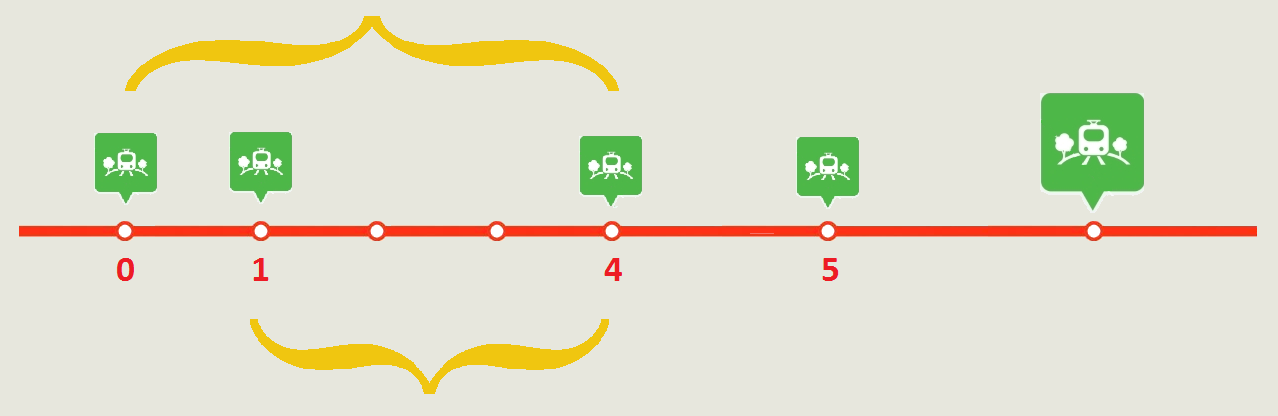
\includegraphics[scale=0.5]{imagenes/ej1/estaciones.png}
	\label{estaciones}
   \end{center}
 \end{figure}

Un algoritmo planteado a partir de esta idea, partiría de la estación Nro. 0 para concluir que se pueden conectar todas desde aquella hasta la Nro 4, para luego continuar revisando una a una las estaciones que pueden unirse partiendo de la Nro 1, cuando resulta evidente que si la distancia entre las estaciones  0 y 4 es menor o igual a la longitud del cable entonces necesariamente la distancia entre la estación siguiente (la Nro. 1) y la Nro. 4 también será menor a la longitud del cable. De no considerar esta premisa se desprende la redundancia en los cálculos que impactan en la complejidad de algoritmo. \\
 
Dicho esto, la propuesta de resolución escogida versa sobre la idea de utilizar información relevada en estaciones anteriores para aminorar la cantidad de cómputos, como se esboza en el siguiente pseudocódigo:

\textcolor{blue}{ME PARECE Q ESTOY SEPARANDO DEL CICLO ALGO Q VA ADENTRO =p}
\begin{algorithmic}

  \IF{Existe alguna estación en el ramal}
    \STATE tomar la primera estación
    \STATE fijarse hasta cuál se puede llegar sin cortar el cable y guardar la estación más lejana alcanzada
    \WHILE{Hay más estaciones}
	\STATE Calcular la distancia entre la estación actual y la más lejana alcanzada
	\IF{La actual no es la última y tampoco lo es la más lejana alcanzada}
		 \STATE Fijarse si alcanza el cable para unir estaciones posteriores a la más lejana conectada hasta el momento, incrementando el contador de estaciones unidas.
	\ENDIF
	\IF { la cantidad de estaciones unidas es mayor al valor máximo alcanzado hasta el momento}
		\STATE actualizar dicho valor
	\ENDIF
   \ENDWHILE
   \STATE Devolver la maxima cantidad de estaciones que se consiguió unir.
  \ELSE
    \STATE Devolver 0
  \ENDIF
\end{algorithmic}

Este procedimiento resolve adecuadamente el problema propuesto porque calcula para cada ciudad inicial la máxima cantidad de ciudades que pueden ser recorridas y lo realiza con una cota de complejidad de O(n).\\


%
%Fijarse si el ramal tiene alguna estacion
%Si tiene:
%	Tomar primera estación
%	Fijarse hasta cuál puede unirse con la longitud del cable dada.
%
%	Mientras haya más estaciones
%		Calcular la distancia entre la estación actual y la más lejana alcanzada
%		Si la actual no es la última & la más lejana alcanzada no es la última
%			Fijarse si alcanza el cable para unir estaciones posteriores a la más lejana conectada hasta el momento
%			incrementando el contador de estaciones unidas.
%		Si la cantidad de estaciones unidas es mayor al valor máximo alcanzado hasta el momento, actualizar dicho 		valor.
%
%	Devolver la maxima cantidad de estaciones que se consiguió unir.
%
%Si no tiene
%	Devolver 0


\subsection{An\'alisis de la complejidad}

\subsection{C\'odigo fuente}

\subsection{Experimentaci\'on}

\subsubsection{Constrastaci\'on Emp\'irica de la complejidad}\label{tiempos}


